% Multi-hop delegation chain walker (Anchor §3).
\documentclass[border=10pt,tikz]{standalone}
\usepackage{tikz}
\usetikzlibrary{arrows.meta,positioning,fit,backgrounds,calc,shapes.symbols,decorations.pathreplacing}

\definecolor{sand}{HTML}{E9DCC4}
\definecolor{sanddeep}{HTML}{D8C7A6}
\definecolor{ebony}{HTML}{121212}
\definecolor{ink}{HTML}{1B1712}
\definecolor{cobalt}{HTML}{003FB8}
\definecolor{amber}{HTML}{6B4500}
\definecolor{teal}{HTML}{00564C}
\definecolor{paper}{HTML}{FBF7EF}

\begin{document}
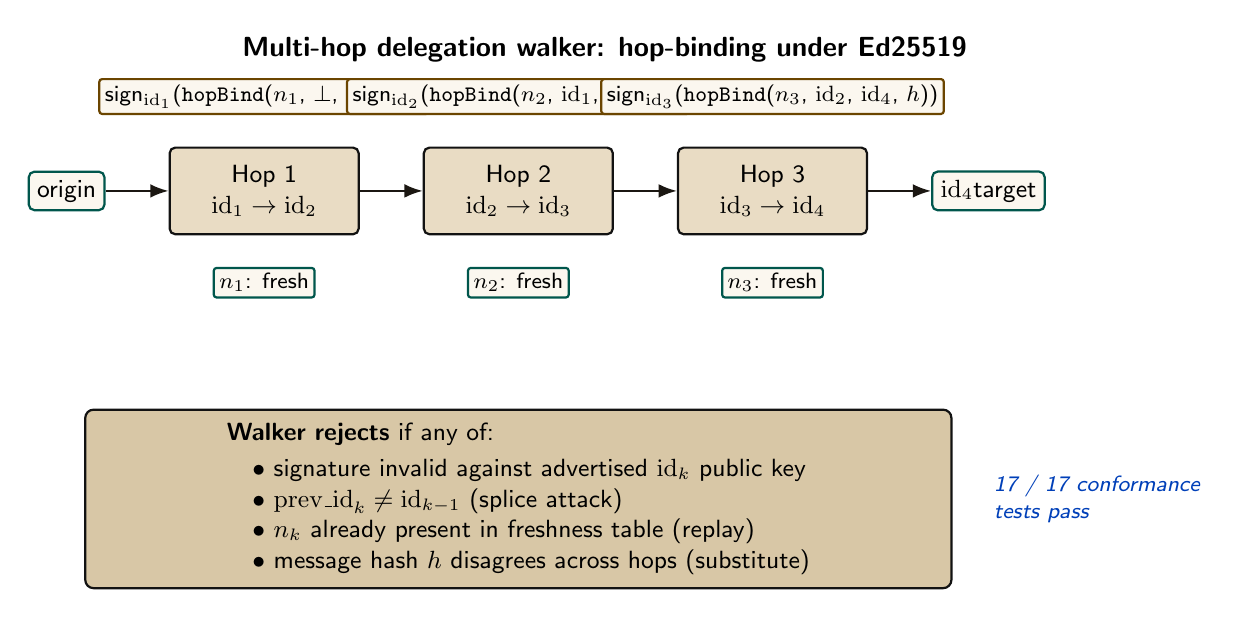
\begin{tikzpicture}[
  font=\sffamily\small,
  hop/.style={draw=ebony,thick,fill=sand,rounded corners=2pt,
              minimum width=24mm,minimum height=11mm,inner sep=3pt,
              align=center},
  sig/.style={draw=amber,thick,fill=paper,rounded corners=1pt,
              inner sep=2pt,font=\sffamily\footnotesize},
  fresh/.style={draw=teal,thick,fill=paper,rounded corners=1pt,
                inner sep=2pt,font=\sffamily\footnotesize},
  arr/.style={->,>=Latex,thick,draw=ink},
  badarr/.style={->,>=Latex,thick,draw=cobalt,dashed},
]

\node[font=\sffamily\bfseries,anchor=west] at (-0.4,4.8)
  {Multi-hop delegation walker: hop-binding under Ed25519};

% Three hops
\node[hop] (h1) at (0,3) {Hop 1\\$\mathrm{id}_1 \to \mathrm{id}_2$};
\node[hop,right=8mm of h1] (h2) {Hop 2\\$\mathrm{id}_2 \to \mathrm{id}_3$};
\node[hop,right=8mm of h2] (h3) {Hop 3\\$\mathrm{id}_3 \to \mathrm{id}_4$};

% Signed bindings (above each hop)
\node[sig,above=4mm of h1,align=center]
  {sign$_{\mathrm{id}_1}$(\texttt{hopBind}($n_1$, $\bot$, $\mathrm{id}_2$, $h$))};
\node[sig,above=4mm of h2,align=center]
  {sign$_{\mathrm{id}_2}$(\texttt{hopBind}($n_2$, $\mathrm{id}_1$, $\mathrm{id}_3$, $h$))};
\node[sig,above=4mm of h3,align=center]
  {sign$_{\mathrm{id}_3}$(\texttt{hopBind}($n_3$, $\mathrm{id}_2$, $\mathrm{id}_4$, $h$))};

% Nonce freshness boxes (below each hop)
\node[fresh,below=4mm of h1] {$n_1$: fresh};
\node[fresh,below=4mm of h2] {$n_2$: fresh};
\node[fresh,below=4mm of h3] {$n_3$: fresh};

% Hop arrows
\draw[arr] (h1.east) -- (h2.west);
\draw[arr] (h2.east) -- (h3.west);

% Terminal arrows
\node[draw=teal,thick,fill=paper,rounded corners=2pt,inner sep=3pt,
      left=8mm of h1] (origin) {origin};
\node[draw=teal,thick,fill=paper,rounded corners=2pt,inner sep=3pt,
      right=8mm of h3] (target) {$\mathrm{id}_4$\\target};
\draw[arr] (origin.east) -- (h1.west);
\draw[arr] (h3.east) -- (target.west);

% Walker verification (below)
\node[draw=ebony,thick,fill=sanddeep,rounded corners=3pt,
      align=left,minimum width=110mm,inner sep=5pt,below=22mm of h2]
      (walker)
  {{\bfseries Walker rejects} if any of:
   \\[2pt]\quad$\bullet$ signature invalid against
       advertised $\mathrm{id}_k$ public key
   \\\quad$\bullet$ $\mathrm{prev\_id}_k \neq \mathrm{id}_{k-1}$
       (splice attack)
   \\\quad$\bullet$ $n_k$ already present in freshness table
       (replay)
   \\\quad$\bullet$ message hash $h$ disagrees across hops
       (substitute)};

% Attack arrow
\node[font=\sffamily\footnotesize\itshape,right=4mm of walker.east,
      align=left,text=cobalt]
  {17 / 17 conformance\\tests pass};

\end{tikzpicture}
\end{document}
